\chapter{\IFRU{BPX: установка прерывания на произвольное место}{BPX: set breakpoint arbitrary point}}

\IFRU{Содержимое регистров процессора будет выведено.}{Content of all CPU registers will be printed.}

\IFRU{Если хотя бы один регистр FPU что-то содержит, он также будет выведен.}{If at least one FPU register contain something, it will be printed too.}

\IFRU{Если содержимое FPU-регистра NaN (нечисло), содержимое регистра FPU будет трактовано как регистра MMX и также будет выведено.}{If the floating point number is also NaN (Not-a-Number), FPU register contents will be treated as MMX register and will be dumped too.}

%\IFRU{Если указана опция \IT{--fpu\_always}, состояние регистров FPU будет выводиться на каждом прерывании.}{If \TT{-fpu\_always} option is set, FPU registers state will be dumped at each breakpoint.}
%*
\IFRU{Если указана опция \IT{--dump-fpu}, состояние регистров FPU будет выводиться.}{If \TT{--dump-fpu} option is set, FPU registers state will be dumped.}
%*
\IFRU{Если указана опция \IT{--dump-xmm}, состояние всех регистров XMM также будет выведено, если только регистр не пуст.}{If \TT{--dump-xmm} option is set, each XMM registers state will be dumped too, unless it is empty.}

\IFRU{\TT{DUMP(ADDRESS|REGISTER|SYMBOL[+OFFSET],SIZE)}: вывод содержимого памяти. Определить адрес в памяти можно в виде шестнадцатиричного значения или в виде \TT{REGISTER+OFFSET}. \TT{SIZE} --- это размер дампа.}{\TT{DUMP(ADDRESS|REGISTER[+OFFSET],SIZE)}: dump contents of memory. Define memory address by hexadecimal address or in form \TT{REGISTER+OFFSET}. \TT{SIZE} is memory dump size.}

\IFRU{Если перед адресом или регистром поставить символ \TT{*}, то tracer вначале прочитает DWORD (или QWORD в x64-версии), примет его за адрес и выдаст дамп по нему. Например: \TT{dump(*ebx,0x100)} --- взять адрес из ячейки памяти на которую указывает регистр ebx и выдать дамп размером 0x100 байт.}{If an asteriks symbol \TT{*} is set before address or register value, then tracer will read DWORD (or QWORD in x64 version), treat it as address and dump a buffer here. For example: \TT{dump(*ebx,0x100)} --- take address on a memory cell EBX register pointing on and dump buffer with size of 0x100 bytes.}

\IFRU{\TT{COPY(ADDRESS|REGISTER|SYMBOL[+OFFSET],C-string)}: скопировать Си-строку по указанному адресу. Си-строка может быть как ASCII-строкой, так и содержать последовательности \TT{\textbackslash{}xXX}, где \TT{XX} --- шестнадцатиричное число. Например: \TT{COPY(EAX,a\textbackslash{}x34\textbackslash{}x56)} --- скопирует три байта 'a', 0x34, и 0x56 по адресу который содержится в EAX.}{\TT{COPY(ADDRESS|REGISTER|SYMBOL[+OFFSET],C-string)}: copy C-string to that address. C-string can be just ASCII-string, but also may contain such sequences like \TT{\textbackslash{}xXX}, where \TT{XX} --- hexadecimal number. For example: \TT{COPY(EAX,a\textbackslash{}x34\textbackslash{}x56)} --- copy 3 bytes 'a', 0x34, and 0x56 to address from EAX register.}

\IFRU{\TT{SET (REGISTER,VALUE)}: записать значение в регистр. EIP/RIP, регистры FPU ST0..ST7 и флаги (PF, SF, AF, ZF, OF, CF, DF) можно модифицировать. Значение трактуется как десятичное число или как число с плавающей запятой, если только не указан префикс 0x.}{\TT{SET (REGISTER,VALUE)}: set register to value. EIP/RIP, FPU registers ST0..ST7 and flags (PF, SF, AF, ZF, OF, CF, DF) are allowed. Value will be treated as decimal or floating point, unless prefix 0x is present.}

\IFRU{Замечание: tracer не модифицирует tag word register в FPU, также он не модифицирует регистр TOP, таким образом, если какой-то регистр FPU маркирован как "пустой" и tracer запишет туда какое-то значение, он останется маркированным как "пустой".}{Note: tracer never modify FPU tag word register as well as not modify TOP register, so, if some FPU register was marked as "empty" and tracer set some value there, it will remain marked "empty".}

\IFRU{Изменение значения регистра EIP/RIP иными словами это передача исполнения в другое место. Это удобно для того чтобы пропускать некоторые куски кода.}{Changing EIP/RIP is on other words is code flow altering. This is useful to bypass some code pieces.}

\section{\IFRU{Примеры}{Examples}}

\subsection{\IFRU{Task Manager: создать иллюзию что у нас 32 или 64 процессора}{Task Manager: make illusion we have 32 or 64 CPUs}}

\IFRU{В}{In} Windows XP SP2 x64 Russian:

\begin{lstlisting}
tracer64.exe -l:c:\windows\system32\taskmgr.exe bpx=0x000000010000A8E4,set(rax,64)
\end{lstlisting}

\IFRU{В}{In} Windows XP SP3 x86 English:

\begin{lstlisting}
tracer.exe -l:c:\windows\system32\taskmgr.exe bpx=0x01006647,set(eax,32)
\end{lstlisting}

\subsection{\IFRU{Перехват развернутой (inline) функции strcmp()}{Inlined strcmp() intercepting}}

\IFRU{Представим что у нас есть такой код который мы компилируем в MS VC 2008:}{Let's imagine we have a code we compile in MS VC 2008:}

\begin{lstlisting}
printf ("%d\n", strcmp("one", "two"));
\end{lstlisting}

\IFRU{После компиляции мы получим:}{After compiling we got:}

\begin{lstlisting}
<pre>
.text:00401000 BA 50 A1 40 00                    mov     edx, offset aTwo ; "two"
.text:00401005 B9 54 A1 40 00                    mov     ecx, offset aOne ; "one"
.text:0040100A 8D 9B 00 00 00 00                 lea     ebx, [ebx+0]
.text:00401010
.text:00401010                   loc_401010:                             ; CODE XREF: _main+2A
.text:00401010 8A 01                             mov     al, [ecx]
.text:00401012 3A 02                             cmp     al, [edx]
.text:00401014 75 29                             jnz     short loc_40103F
.text:00401016 84 C0                             test    al, al
.text:00401018 74 12                             jz      short loc_40102C
.text:0040101A 8A 41 01                          mov     al, [ecx+1]
.text:0040101D 3A 42 01                          cmp     al, [edx+1]
.text:00401020 75 1D                             jnz     short loc_40103F
.text:00401022 83 C1 02                          add     ecx, 2
.text:00401025 83 C2 02                          add     edx, 2
.text:00401028 84 C0                             test    al, al
.text:0040102A 75 E4                             jnz     short loc_401010
.text:0040102C
.text:0040102C                   loc_40102C:                             ; CODE XREF: _main+18
.text:0040102C 33 C0                             xor     eax, eax
.text:0040102E 50                                push    eax
.text:0040102F 68 58 A1 40 00                    push    offset byte_40A158 ; char *
.text:00401034 E8 1C 00 00 00                    call    _printf
.text:00401039 83 C4 08                          add     esp, 8
.text:0040103C 33 C0                             xor     eax, eax
.text:0040103E C3                                retn
\end{lstlisting}

\IFRU{Давайте перехватим эту развернутую функцию strcmp и выведем то на что указывают регистры ECX и EDX:}{Let's intercept inlined strcmp function and dump what is at ECX and EDX:}

\begin{lstlisting}
tracer.exe -l:strcmp.exe bpx=8A013A02752984C074128A41013A4201751D83C10283C20284C075E433C0,dump(ecx,0x10),dump(edx,0x10)
\end{lstlisting}

\IFRU{Получим:}{We got:}

\begin{lstlisting}
bytemask_0 is resolved to address 0x401010 (strcmp.exe)
TID=6436|(0) 0x401010 (strcmp.exe!BASE+0x1010)
EAX=0x007722E0 EBX=0x7EFDE000 ECX=0x0040A154 EDX=0x0040A150
ESI=0x00000000 EDI=0x00000000 EBP=0x0018FF88 ESP=0x0018FF44
EIP=0x00401010
FLAGS=PF ZF IF
Dumping memory at ECX
0040A154: 6F 6E 65 00 25 64 0A 00-28 00 6E 00 75 00 6C 00 "one.%d..(.n.u.l."
Dumping memory at EDX
0040A150: 74 77 6F 00 6F 6E 65 00-25 64 0A 00 28 00 6E 00 "two.one.%d..(.n."
\end{lstlisting}

\IFRU{Замечание: только первое вхождение при поиске байтмаски будет использоваться.}{Note: only first bytemask occurence will be intercepted.}

\subsection{\IFRU{Изменение флагов перед тем как условный переход будет совершен}{Change flags before conditional dump is taken}}

\begin{lstlisting}
tracer64.exe -l:flags.exe bpx=0x140001014,set(zf,1)
\end{lstlisting}

\IFRU{Замечание: момент когда tracer меняет состояние регистров это момент \IT{перед} тем как текущая инструкция будет исполнена. Изменение флагов \IT{перед} инструкциями TEST или CMP бессмысленно.}{Note: the moment when tracer can change registers state is the moment \IT{before} current instruction is executed. Changing flags \IT{before} TEST or CMP instructions is useless.}

\subsection{\IFRU{Шутка в Microsoft Excel}{Microsoft Excel practical joke}}

\IFRU{Сделать 666 результатом всех операций деления. Введите "=(123/456)" для проверки.}{Make result of all divisions 666. Enter "=(123/456)" to check.}

\IFRU{Работает для Excel.exe версии}{Works for Excel.exe version} 14.0.4756.1000 (Microsoft Office 2010)

\begin{lstlisting}
tracer.exe -l:excel.exe bpx=excel.exe!base+0x11E91B,set(st0,666)
\end{lstlisting}

\begin{lstlisting}
tracer64.exe -l:excel.exe bpx=excel.exe!base+0x1B7FCC,set(st0,666)
\end{lstlisting}

\IFRU{(Указанный адрес это место после инструкции FDIV, которая собственно и производит деление)}{(The address there is the point after FDIV instruction actually do division here)}

\begin{figure}[ht!]
\centering
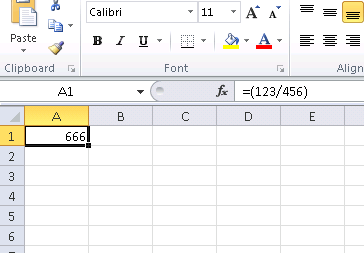
\includegraphics[scale=0.66]{excel_prank.png}
\caption{excel\_prank.png}
\end{figure}

